%% Real-Time Symbolic Dynamic Programming -> AAAI15 Camera -Ready
%% V1.0
%% 2014/11/1
%% by Luis Gustavo Rocha Vianna
\documentclass[letterpaper]{article}

% Required Packages
\usepackage{aaai}
\usepackage{times}
\usepackage{helvet}
\usepackage{courier}
\setlength{\pdfpagewidth}{8.5in}
\setlength{\pdfpageheight}{11in}

% Table
\usepackage{booktabs}
\usepackage{multirow}

% PDFINFO for PDFLATEX
\pdfinfo{
/Title (Real-Time Symbolic Dynamic Programming)
/Author (Luis Vianna, Scott Sanner, Leliane Nunes de Barros)
/Keywords (Hybrid MDPs, Continuous Planning, Symbolic Dynamic Programming)
}

% Section Numbers
%\setcounter{secnumdepth}{0}


% Title, Author, and Address Information
\title{Real-Time Symbolic Dynamic Programming for Hybrid MDPs}

%\author{Anonymous}
\author{
Luis G. R. Vianna \and Leliane N. de Barros\\
IME - USP\\
S\~ao Paulo, Brazil\\
\And
Scott Sanner\\
NICTA \& ANU\\
Canberra, Australia}

\usepackage[pdftex]{graphicx}
\usepackage[cmex10]{amsmath}
\usepackage{amssymb}
\usepackage[vlined,algoruled,linesnumbered,titlenumbered]{algorithm2e}
\usepackage[]{subfig}

\newcommand{\solutionExample}{inventory2Value}
\newcommand{\perfOne}{reservoir3convergence}
\newcommand{\perfTwo}{inventory3convergence}
\newcommand{\perfThree}{traffic1convergence}
\newcommand{\Invent}{\textsc{Inventory Control}}
\newcommand{\Traffic}{\textsc{Traffic Control}}
\newcommand{\Reservoir}{\textsc{Reservoir Management}}
\def\argmax{\operatornamewithlimits{arg~max}}
\def\argmin{\operatornamewithlimits{arg~min}}
\def\pmax{\operatornamewithlimits{pmax}}
 \hbadness = 2000

\begin{document}
\maketitle

\begin{abstract}
Recent advances in Symbolic Dynamic Programming (SDP) combined with
the extended algebraic decision diagram (XADD) have provided exact
solutions for expressive subclasses of finite-horizon Hybrid Markov
Decision Processes (HMDPs) with mixed continuous and discrete state
and action parameters.  Unfortunately, SDP suffers from two major
drawbacks: (1) it solves for all states and can be intractable for
many problems that inherently have large optimal XADD value function
representations; and (2) it cannot maintain compact (pruned) XADD
representations for domains with nonlinear dynamics and reward due to
the need for nonlinear constraint checking.  In this work, we
simultaneously address both of these problems by introducing real-time
SDP (RTSDP).  RTSDP addresses (1) by focusing the solution and value
representation only on regions reachable from a set of initial states
and RTSDP addresses (2) by using visited states as witnesses of
reachable regions to assist in pruning irrelevant or unreachable
(nonlinear) regions of the value function.  To this end, RTSDP enjoys
provable convergence over the set of initial states and substantial
space and time savings over SDP as we demonstrate in a variety of 
hybrid domains ranging from inventory to reservoir to traffic control.
\end{abstract}

%%%%%%%%%%%%%%%%%%%%%%%%%%%%%%%%%%%%%%%%%%%%%%%
\section{Introduction}

Real-world planning applications frequently involve continuous resources (e.g. water, energy and speed) and can be modelled as Hybrid Markov Decision Processes (HMDPs). Problem 1 is an example of an HMDP representing the \Reservoir~ problem, where the water levels are continuous variables.
%Most existing exact solutions for HMDPs make restrictive assumptions of hyper-rectangular partitions~(\cite{feng04,li05}) or use approximate projections on continuous base functions~(\cite{li05,kveton06HALP}).
%sanner11
Symbolic dynamic programming (SDP)~(\cite{zamani12}) provides an exact solution for finite-horizon HMDPs with mixed continuous and discrete state and action parameters, using the eXtended Algebraic Decision Diagram (XADD) representation.
The XADD structure is a generalisation of the algebraic decision diagram (ADD)~\cite{bahar93add} to compactly represent functions of both discrete and continuous variables.
Decision nodes may contain boolean variables or inequalities between expressions containing continuous variables.
Terminal nodes contain an expression on the continuous variables which could be evaluated to a real number.
An XADD representation of the reward function of \Reservoir~ is shown in Figure \ref{fig:exampleDD}.

%%%%%%%%%%%%%%%%%%%%%%%%%%%%%%%%%%%%%%%%%%%%%%%%
\begin{figure}[t!]
\begin{minipage}{0.25\textwidth}
\center
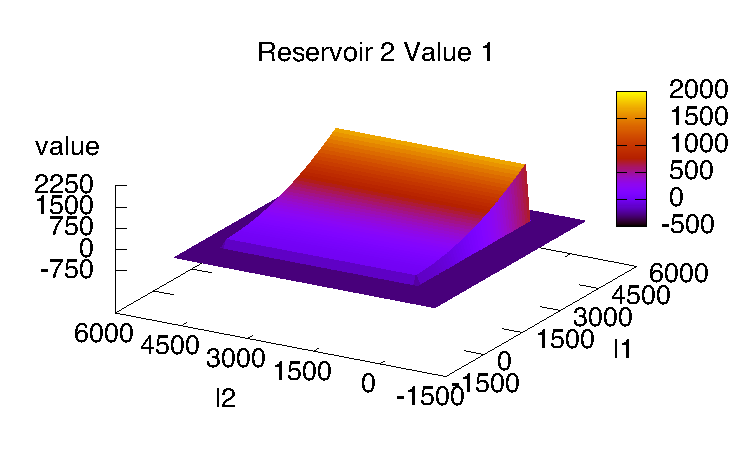
\includegraphics[width=\textwidth, height=0.8\textwidth]{figures/reservoir2Value1/reservoir2Value1.pdf} 
\end{minipage}
\begin{minipage}{0.20\textwidth}
\center
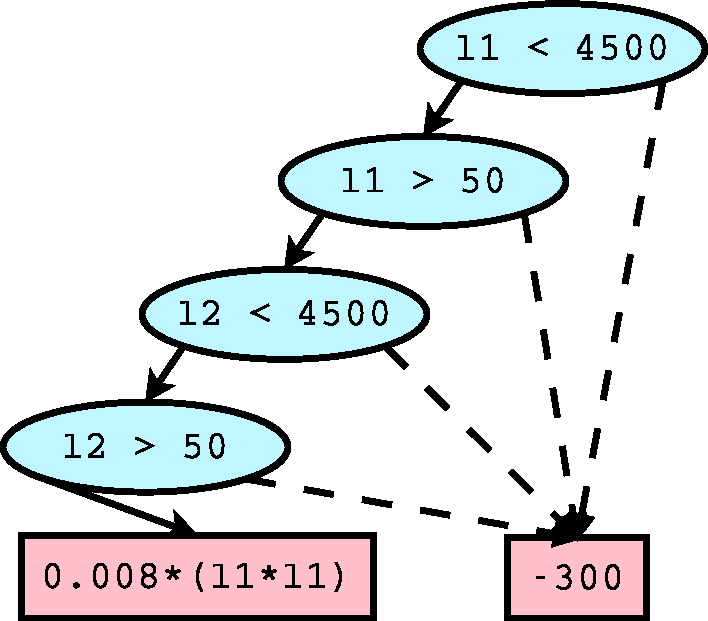
\includegraphics[width=\textwidth, height=0.8\textwidth]{figures/reservoir2Value1/reservoir2Value1DD.pdf}
\end{minipage}
\caption{\small Nonlinear reward function for the \Reservoir~ domain: graphical plot~\emph{(left)}; XADD representation~\emph{(right)}: blue ovals are internal nodes, pink rectangles are terminal nodes, $true$ branches are solid lines and $false$ are dashed.}
\label{fig:exampleDD}
\end{figure}
%%%%%%%%%%%%%%%%%%%%%%%%%%%%%%%%%%%%%%%%%%%%%%%%
\paragraph{\bf Problem 1 - \Reservoir~\cite{Yeh1985,Mahootchi2009}. \label{ex1}}
\textit{
In this problem, the task is to manage a water supply reservoir chain made up of $k$ reservoirs each with a continuous water level $L_i$.
The $drain_i$ and $no$-$drain_i$ actions determine whether water is drained from reservoir $i$ to the next.
The amount of drained water is linear on the water level, and the amount of energy produced is proportional to the product of drained water and water level.
At every iteration, the top reservoir receives a constant spring replenishment plus a non-deterministic rain while the bottom reservoir has a part of its water used for city purposes. For example, the water level of the top reservoir, $L_1$, at the next iteration is:
{\small
\hspace{-2mm}
\begin{align}
L_1' =
\begin{cases}
  \text{if }  rain \wedge drain_1 &\hspace{-2mm}: L_1 + 1000 - 0.5L_1\\ 
  \text{if }  \neg rain \wedge drain_1 &\hspace{-2mm}: L_1 + 500 - 0.5L_1\\ 
  \text{if }  rain \wedge \neg drain_1 &\hspace{-2mm}: L_1 + 1000\\ 
  \text{if }  \neg rain \wedge \neg drain_1 &\hspace{-2mm}: L_1 + 500\\ 
\end{cases}
\label{eq:l1}
\end{align}
}
A {\bf nonlinear} reward is obtained by generating energy and there is a strong penalty if any reservoir level is outside the nominal minimum and maximum levels.
{\small
\begin{align*}
R_{drain_i} (L_i)=
\begin{cases}
  \text{if }  50 \leq L_i \leq 4500 &\hspace{-2mm} : 0.008\cdot L_i^2\\ 
  \text{else}  &\hspace{-2mm} : -300\\ 
\end{cases}
\end{align*}
}
}

Unfortunately, SDP solutions for HMDPs suffer from two major drawbacks: (1) the overhead of computing a complete optimal policy even for problems where the initial state is known; and (2) it cannot maintain compact (pruned) XADD representations of functions containing nonlinear decisions because it cannot verify their feasibility and remove or ignore infeasible regions.
In this work, we address both of these problems simultaneously by proposing a new HMDP solver, named \emph{Real-Time Symbolic Dynamic Programming (RTSDP)}.
RTSDP addresses (1) by restricting the solution to states relevant to a specified initial state and addresses (2) by only expanding regions containing visited states, thus ignoring infeasible branches of nonlinear decisions. The RTSDP solution is focused on the initial state by using simulation trials as done in Real-Time Dynamic Programming (RTDP).

We use the Real-Time Dynamic Programming (RTDP) algorithm because it is considered a state-of-the-art solver for MDPs~\cite{Barto95RTDP,kolobov12GOURMAND} that combines initial state information and value function heuristics with asynchronous updates to generate an optimal partial policy for the relevant states, i.e., states reachable from the initial state following an optimal policy.
In order to be used in a hybrid state space, RTSDP modifies RTDP's single state update to a \emph{region based} symbolic update. The XADD representation naturally factors the state-space into regions with the same continuous expressions, and thus allows efficient \emph{region based updates} that improve the value function  \emph{on all states in the same region}. We claim that region updates promote better reusability of previous updates, improving the search efficiency. 
RTSDP is empirically tested on three challenging domains: \Invent, with continuously parametrized actions; \Reservoir, with a nonlinear reward model; and \Traffic, with nonlinear dynamics.
Our results show that, given an initial state, RTSDP can solve finite-horizon HMDP problems faster and using far less memory than SDP.

%%%%%%%%%%%%%%%%%%%%%%%%%%%%%%%%%%%%%%%%%%%%%%%
\section{Hybrid Markov Decision Processes}

An MDP~\cite{puterman94} is defined by: a set of states $\mathcal{S}$, actions $\mathcal{A}$, a probabilistic transition function $\mathcal{P}$ and a reward function $\mathcal{R}$.
In HMDPs, we consider a model factored in terms of variables~\cite{boutilier99}, i.e.
a state $s \in \mathcal{S}$ is a pair of assignment vectors $(\vec{b},\vec{x})$, where $\vec{b} \in \{ 0,1 \}^n$ is boolean variables vector and each $\vec{x} \in \mathbb{R}^m$ is continuous variables vector, and the action set $\mathcal{A}$ is composed by a finite set of parametric actions, i.e. $\mathcal{A} = \{ a_1(\vec{y}), \ldots, a_K(\vec{y})\}$, where $\vec{y}$ is the vector of parameter variables.
The functions of state and action variables are compactly represented by exploiting structural independencies among variables in dynamic Bayesian networks (DBNs)~\cite{dean90DBN}. 

We assume that the factored HMDP models satisfy the following: (i) next state boolean variables are probabilistically dependent on previous state variables and action; (ii) next state continuous variables are deterministically dependent on previous state variables, action and current state boolean variables; (iii) transition and reward functions are piecewise polynomial in the continuous variables. 
These assumptions allow us to write the probabilistic transition function $\mathcal{P}(s' | a(\vec{y}),s)$ in terms of state variables, i.e.:

{\small
\begin{equation*}
\hspace{-0.6mm} \mathcal{P}(\vec{b'},\vec{x'} | a(\vec{y}),\vec{b},\vec{x}) =\hspace{-0.2mm} \prod_{i=1}^{n} \mathcal{P}(b_i' | a(\vec{y}),\vec{b},\vec{x}) \prod_{j=1}^{m} \mathcal{P}(x_j' | \vec{b'}, a(\vec{y}),\vec{b},\vec{x}).\hspace{-2mm}
\end{equation*}
}

Assumption (ii) implies the conditional probabilities for continuous variables are Dirac Delta functions, which correspond to conditional deterministic transitions: $x'_i \gets T^i_{a(\vec{y})}(\vec{b},\vec{x},\vec{b'})$. An example of conditional deterministic transition is given in Problem 1, the definition of $L'_1$ in Equation \ref{eq:l1}.
Though this restricts stochasticity to boolean variables, continuous variables depend on their current values, allowing the representation of general finite distributions, a common restriction in exact HMDP solutions~\cite{feng04,meuleau09HAO,zamani12}.

In this paper, we consider finite-horizon HMDPs with an initial state $s_0 \in \mathcal{S}$ and horizon $H \in \mathbb{N}$.
A non-stationary policy $\pi$ is a function which specifies the action $a(\vec{y}) = \pi(s, h)$ to take in state $s \in \mathcal{S}$ at step $h \leq H$.
The solution of an HMDP planning problem is an optimal policy $\pi^*$ that maximizes the expected accumulated reward, i.e.:%, $V^{\pi^*}(s_0)$:
{\small
\begin{equation*}
V_{H}^{\pi^*}(s_0)= \mathbb{E} \left[ \sum_{t=1}^{H} \mathcal{R}(s_t, a_t(\vec{y_t})) \Big| s_{t+1} \sim \mathcal{P}(s'|a_t(\vec{y_t}),s_{t}) \right], %\label{eq:vfun_def}
\end{equation*}
}
where $a_t(\vec{y_t}) = \pi^*(s_t,t)$ is the action chosen by $\pi^*$.

%%%%%%%%%%%%%%%%%%%%%%%%%%%%%%%%%%%%%%%%%%%%%%%
\section{Symbolic Dynamic Programming}

The symbolic dynamic programming (SDP) algorithm~\cite{sanner11,zamani12} is a generalisation of the classical {\it value iteration} dynamic programming algorithm~\cite{bellman57} for constructing optimal policies for Hybrid MDPs.
It proceeds by constructing a series of $h$ stages-to-go optimal value functions $V_h(\vec{b},\vec{x})$.
The pseudocode of SDP is shown in Algorithm \ref{alg:sdp}.
Beginning with $V_0(\vec{b},\vec{x}) = 0$ (line 1), it obtains the \emph{quality} $Q_{h,a(\vec{y})}(\vec{b},\vec{x})$ for each action $a(\vec{y}) \in \mathcal{A}$ (lines 4-5) in state $(\vec{b},\vec{x})$ by regressing the expected reward for $h-1$ future stages $V_{h-1}(\vec{b},\vec{x})$ along with the immediate reward $R(\vec{b},\vec{x},a(\vec{y}))$ as the following:
{\small
\begin{align}
Q_{h,a(\vec{y})}(\vec{b},\vec{x}) =  R(\vec{b},\vec{x},a(\vec{y})) + \sum_{\vec{b}'} \int_{\vec{x}'} \Bigg[ 
\prod_i \mathcal{P}(b_i' | a(\vec{y}),\vec{b},\vec{x}) \cdot \nonumber 
\end{align}

\begin{align}
\hspace{20mm} \prod_j \mathcal{P}(x_j' | \vec{b'}, a(\vec{y}),\vec{b},\vec{x})\cdot V_{h-1}(\vec{b}',\vec{x}') \Bigg]. \label{eq:sdpregr} 
\end{align}
}
Note that since we assume deterministic transitions for continuous variables the integral over the continuous probabilistic distribution is actually a substitution:
$$
 \int_{\vec{x_i}'} \mathcal{P}(x_i' | \vec{b'}, a(\vec{y}),\vec{b},\vec{x}) \cdot f(x_i') =
subst_{x_i' = T^i_{a(\vec{y})}(\vec{b},\vec{x},\vec{b'})} f(x_i') 
$$
Given $Q_{h,a(\vec{y})}(\vec{b},\vec{x})$ for each $a(\vec{y}) \in A$, we can define the $h$ stages-to-go value function as the quality of the best (greedy) action in each state $(\vec{b},\vec{x})$ as follows (line 6):
\begin{align}
V_{h}(\vec{b},\vec{x}) & = \max_{a(\vec{y}) \in A} \left\{ Q_{h,a(\vec{y})}(\vec{b},\vec{x}) \right\}. \label{eq:sdpmax}
\end{align}

The optimal value function $V_h(\vec{b},\vec{x})$ and optimal policy $\pi^*_h$ for each stage $h$ are computed after $h$ steps. Note that the policy is obtained from the maximization in Equation~\ref{eq:sdpmax}, $\pi^*_h(\vec{b},\vec{x})$ $=$ $\argmax_{a(\vec{y})} Q_{h,a(\vec{y})}(\vec{b},\vec{x})$ (line 7). 

%%%%%%%%%%%%%%%%%%%%%%%%%%%%%%%%%%%%%%%%%%%%%%%
\begin{algorithm}[ht!]
%\scriptsize
\footnotesize
\DontPrintSemicolon
\caption{\small \texttt{SDP}(HMDP M, $H$) $\rightarrow$ $(V^h,\pi^*_h)$ \\\cite{zamani12}\label{alg:sdp}}
\SetKwFunction{regress}{Regress}
\SetKwFunction{myproc}{\bf Procedure}{}{}
\SetKwFunction{remapWithPrimes}{Prime}
	$V_0:=0, h:=0$\;
	\While{$h < H$}{
		$h:=h+1$\;
		\ForEach {$a \in A$}{
			$Q_{a(\vec{y})} \gets\,$\regress{$V_{h-1},{a(\vec{y})}$}\;
		}
		$V_{h} \! \gets \! \max_{a(\vec{y})} \, Q_{a(\vec{y})}$ $\,$ \emph{// Maximize all $Q_{a(\vec{y})}$}\;
		$\pi^*_h \gets \argmax_{a(\vec{y})} \, Q_{a(\vec{y})} $\;
	}
	\Return{$(V_h, \pi^*_h)$} \;
\vspace{3mm}

%\setcounter{AlgoLine}{0}
\myproc~{\bf 1.1}:~\regress{$V_{h-1}$, $a(\vec{y})$ }{

$Q=$ \remapWithPrimes{$V_{h-1}$} $\,$ \emph{// Rename all symbolic variables} 
- \hspace{25mm} \emph{// $b_i \to b_i'$ and all $ x_i \to x_i'$} \;
\ForEach { $b_i'$ in $Q$}  
    {
	\emph{// Discrete marginal summation, also denoted $\sum_{b'}$}\\
	$Q \gets \left[ Q \otimes P(b_i'|\vec{b},\vec{x},a(\vec{y})) \right]|_{b_i' = 1}$
	\mbox{$\;\;\;\;\;\;\;$}$\oplus \left[ Q \otimes P(b_i'|\vec{b},\vec{x},a(\vec{y})) \right]|_{b_i' = 0}$\;
}
	\ForEach { $x_j'$ in $Q$}  
{
	\emph{//Continuous marginal integration}\\
	$Q \gets subst_{x'_j = T_{a(\vec{y})}(\vec{b},\vec{x},\vec{b'})} Q $\;
}
	\Return{$Q \oplus R(\vec{b},\vec{x},a(\vec{y}))$}\;
}
\end{algorithm}
%%%%%%%%%%%%%%%%%%%%%%%%%%%%%%%%%%%%%%%%%%%%%%%

\subsection{XADD representation}

XADDs~\cite{sanner11} are directed acyclic graphs that efficiently represent and manipulate piecewise polynomial functions by using decision nodes for separating regions and terminal nodes for the local functions.
Internal nodes are decision nodes that contain two edges, namely \emph{true} and \emph{false} branches, and a decision that can be either a boolean variable or a polynomial inequality on the continuous variables.
Terminal nodes contain a polynomial expression on the continuous variables.
Every path in an XADD defines a partial assignment of boolean variables and a continuous region.

%For example, Figure~\ref{fig:exampleDD}(left) shows the plot of a piecewise function and Figure~\ref{fig:exampleDD}(right) its XADD representation.
%that satisfies all inequalities in its internal nodes.
%If there are many regions with the same local function, then the paths will merge into a single terminal node, as in the dashed lines of Figure~\ref{fig:exampleDD} (right). 

The SDP algorithm uses four kinds of XADD operations~\cite{sanner11,zamani12}:
(i) \emph{Algebraic operations} (sum $\oplus$, product $\otimes$), naturally defined within each region, so the resulting partition is a cross-product of the original partitions;% (See Figure \ref{fig:XADDadd}),
(ii) \emph{Substitution operations}, which replace or instantiate variables by modifying expressions on both internal and terminal nodes.(See Figure \ref{fig:XADDsubs});
(iii) \emph{Comparison operations} (maximization), which cannot be performed directly between terminal nodes so new decision nodes comparing terminal expressions are created (See Figure \ref{fig:XADDmax});
(iv) \emph{Parameter maximization operations}, (\emph{pmax} or $\max_{\vec{y}}$) remove parameter variables from the diagram by replacing them with values that maximize the expressions in which they appear. (See Figure \ref{fig:XADDparamax}).
%These XADD operations have been defined previously and we refer to for details.
%%%%%%%%%%%%%%%%%%%%%%%%%%%%%%%%%%%%%%%%%%%%%%%
\begin{figure}[th]
\center
%\subfloat[Addition~($\oplus$).]{
%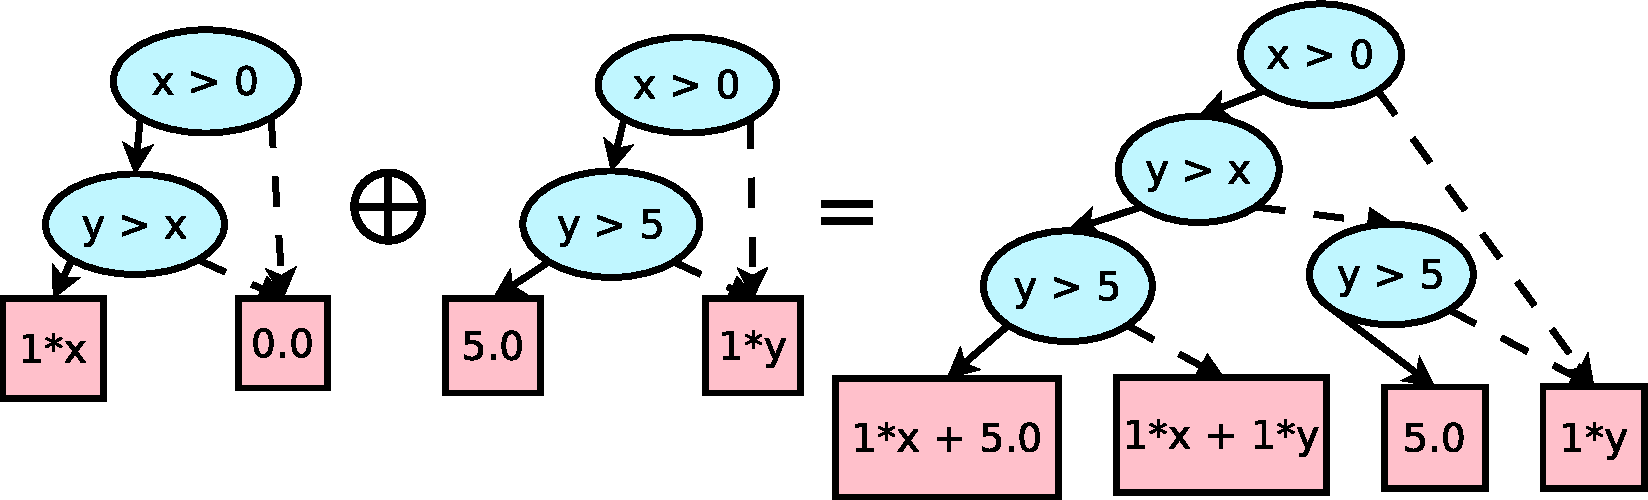
\includegraphics[width=0.45\textwidth]{figures/xaddOps/XADDsum.pdf} 
%\label{fig:XADDadd}
%}

\hspace{10mm}
\subfloat[Substitution~($subst$).]{
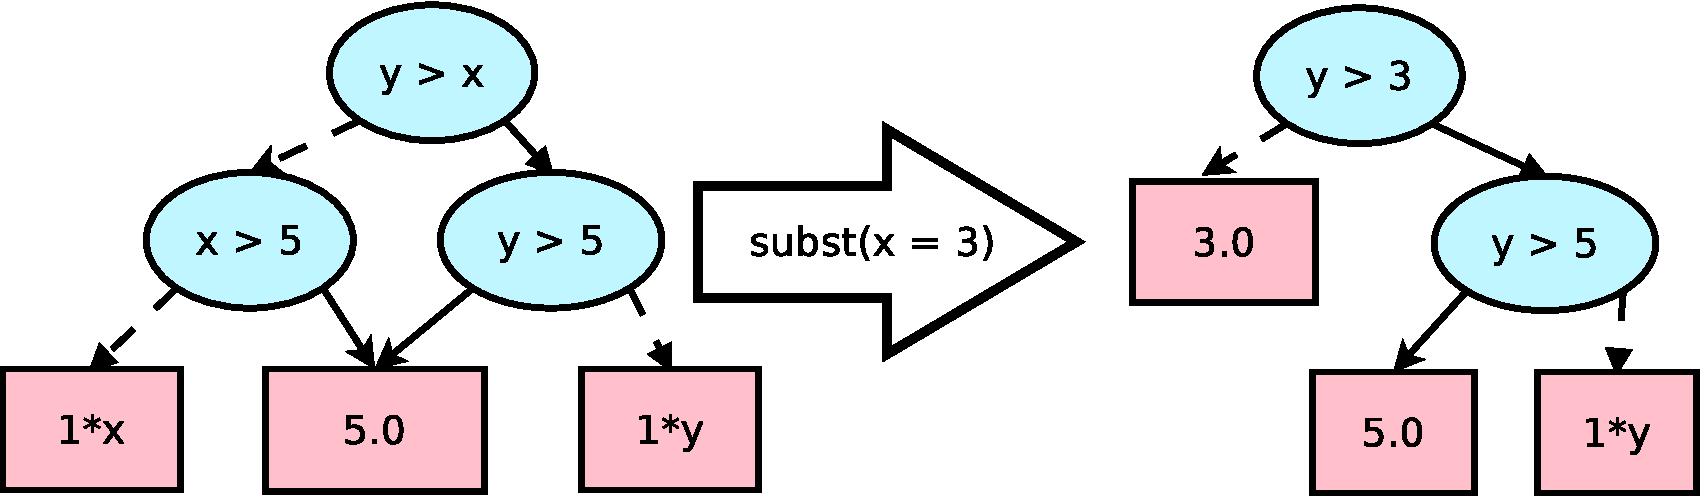
\includegraphics[width=0.37\textwidth]{figures/xaddOps/XADDsubs.pdf} 
\label{fig:XADDsubs}
}

\subfloat[Maximization~($\max$)]{
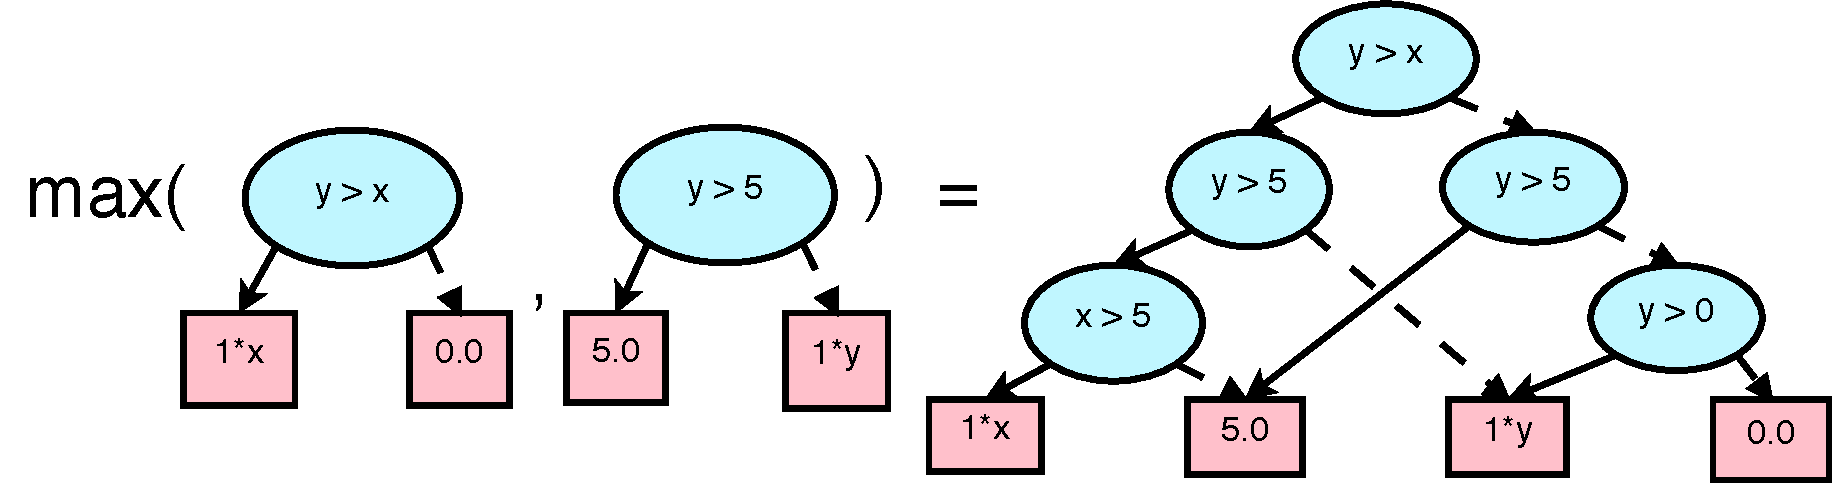
\includegraphics[width=0.46\textwidth]{figures/xaddOps/XADDmax.pdf} 
\label{fig:XADDmax}
}

\subfloat[Parameter Maximization~($\pmax$).]{
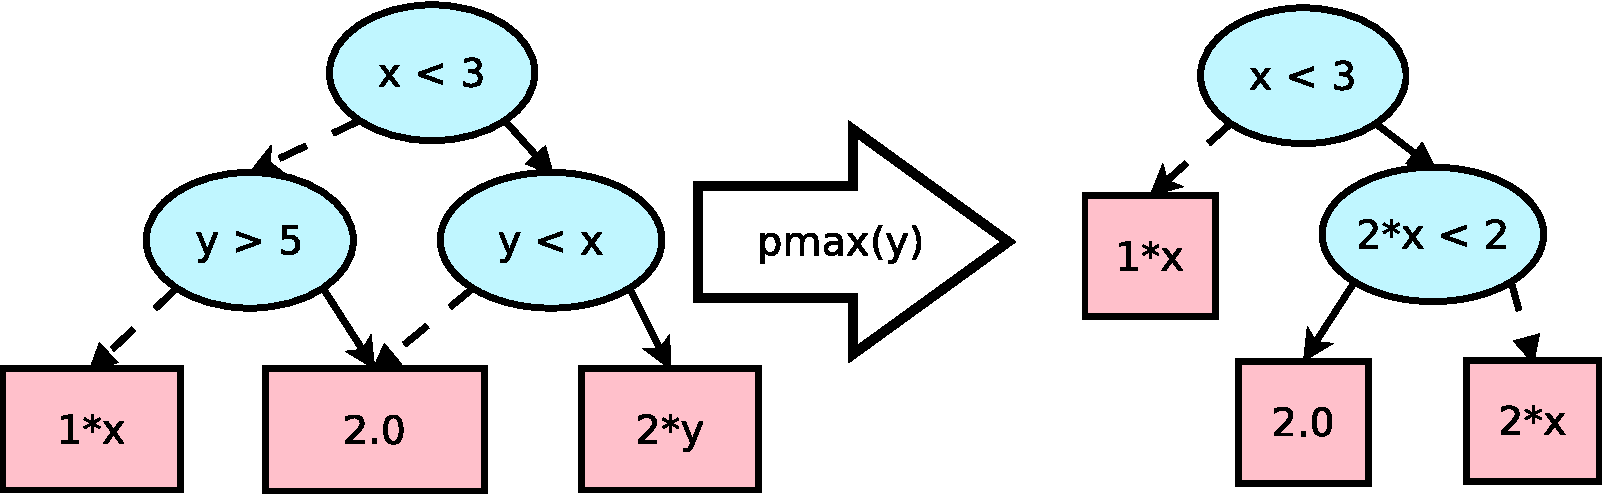
\includegraphics[width=0.4\textwidth]{figures/xaddOps/XADDpmax.pdf} 
\label{fig:XADDparamax}
}
\caption{Examples of basic XADD operations.}
\end{figure}
%%%%%%%%%%%%%%%%%%%%%%%%%%%%%%%%%%%%%%%%%%%%%%%

Thus, the SDP Bellman update (Equations \ref{eq:sdpregr} \& \ref{eq:sdpmax}) is performed synchronously as a sequence of XADD operations \footnote{$F^{DD(vars)}$ is a notation to indicate that $F$ is an XADD symbolic function of $vars$.}, in two steps:
\begin{itemize}
\item {Regression of action $a$ for all states:
{\small
\begin{align}
Q_{h,a}^{DD(\vec{b},\vec{x},\vec{y})} & =  R_a^{DD(\vec{b},\vec{x},\vec{y})} \oplus \nonumber \\
	& \hspace{-1.4cm}  \sum_{\vec{b}'}  P_a^{DD(\vec{b},\vec{x},\vec{y},\vec{b'})} \otimes \left[ subst_{(x' = T_a^{DD(\vec{b},\vec{x},\vec{y},\vec{b'})})} V_{h-1}'^{DD(b',x')} \right]. 
\label{eq:SDPregrDD}
\end{align}
}
}
\item{
Maximization for all states w.r.t. the action set $\mathcal{A}$:
\begin{equation}
V_h^{DD(\vec{b},\vec{x})} = \max_{a\in\mathcal{A}} \left( \max_{\vec{y}}~ Q_{h,a}^{DD(\vec{b},\vec{x},\vec{y})} \right).
\label{eq:SDPmaxDD}
\end{equation}
}
\end{itemize}

As these operations are performed the complexity of the value function increases and so does the number of regions and nodes in the XADD. A goal of this work is to propose an efficient solution that avoids exploring unreachable or unnecessary regions.

%%%%%%%%%%%%%%%%%%%%%%%%%%%%%%%%%%%%%%%%%%%%%%%
\section{Real-Time Symbolic Dynamic Programming}

First, we describe the RTDP algorithm for MDPs which motivates the RTSDP algorithm for HMDPs.

\subsection{The RTDP algorithm}

The RTDP algorithm~\cite{Barto95RTDP} (Algorithm \ref{alg:rtdp}) starts from an initial admissible heuristic value function $V$ ($V(s) > V^*(s), \forall s$) and performs trials to iteratively improve by monotonically decreasing the estimated value. A trial, described in Procedure 2.1, is a simulated execution of a policy interleaved with local Bellman updates on the visited states.
Starting from a known initial state, an update is performed, the greedy action is taken, a next state is sampled and the trial goes on from this new state. Trials are stopped when their length reaches the horizon $H$.

The update operation (Procedure 2.2) uses the current value function $V$ to estimate the future reward and evaluates every action $a$ on the current state in terms of its quality $Q_a$. The greedy action, $a_g$, is chosen and the state's value is set to $Q_{a_g}$.
RTDP performs updates on one state at a time and only on relevant states, i.e. states that are reachable under the greedy policy. Nevertheless, if the initial heuristic is admissible, there is an optimal policy whose relevant states are visited infinitely often in RTDP trials. Thus the value function converges to $V^*$ on these states and an optimal partial policy closed for the initial state is obtained. As the initial state value depends on all relevant states' values, it is the last state to convergence.

%%%%%%%%%%%%%%%%%%%%%%%%%%%%%%%%%%%%%%%%%%%%%%%
\begin{algorithm}[th!]
\footnotesize
\DontPrintSemicolon
\caption{\small \texttt{RTDP}(MDP $\mathit{M}$, $s_0$, $H$, $V$) $\longrightarrow$ $V^*_H(s_0)$ \label{alg:rtdp}}
\SetKwFunction{maketrial}{MakeTrial}
\SetKwFunction{timeout}{TimeOut}
\SetKwFunction{solved}{Solved}
\SetKwFunction{update}{Update}
\SetKwFunction{sample}{Sample}
\SetKwFunction{myproc}{\bf Procedure}

\While{$\neg~\solved(M,s_0,V) \wedge \neg \timeout() $}{
	$V \gets \maketrial(\mathit{M}, s_0, V, H)$\;
	}
     \Return{$V$} \;
\vspace{4mm}

%\setcounter{AlgoLine}{0}
\myproc~{\bf 2.1}:~\maketrial{MDP $\mathit{M}$, $s$, $V$, $h$}{

	\If {$s \in GoalStates$ or $h = 0$} {\Return {$V$}}
	$V_h(s), a_g \gets \update(M, s, V, h)$\;
	// Sample next state from $P(s, a, s')$\;
	$s^{new} \gets \sample(s, a_g, \mathit{M})$ \;
	\Return {$\maketrial(\mathit{M}, s^{new}, V, h-1)$}\;
}
\vspace{4mm}

%\setcounter{AlgoLine}{0}
\myproc~{\bf 2.2}:~\update{MDP $\mathit{M}$, $s$, $V$, $h$}{

\ForEach {$a \in A$}{
              $Q_{a} \gets R(s, a) + \sum_{s' \in S} P(s, a, s') \cdot \left[V_{h-1}(s') \right] $\;
    }
    $a_g \gets \argmax_a Q_a$\;
    $V_h(s) \gets Q_{a_g}$\;
    \Return {$V_h(s), a_g$}\;
}
\end{algorithm}
%%%%%%%%%%%%%%%%%%%%%%%%%%%%%%%%%%%%%%%%%%%%%%%

\subsection{The RTSDP Algorithm}

We now generalize the RTDP algorithm for HMDPs.
The main \texttt{RTDP} (Algorithm \ref{alg:rtdp}) and \texttt{makeTrial} (Procedure 2.1) functions are trivially extended as they are mostly independent of the state or action structure, for instance, verifying if current state is a goal is now checking if the current state belongs to a goal region instead of a finite goal set. %structure.
The procedure that requires a non-trivial extension is the \texttt{Update} function (Procedure 2.2).
Considering the continuous state space, it is inefficient to represent values for individual states, therefore we define a new type of update, named \emph{region update}, which is one of the contributions of this work.

While the synchronous SDP update (Equations \ref{eq:SDPregrDD} and \ref{eq:SDPmaxDD}) modifies the expressions for all paths of $V^{DD(\vec{b},\vec{x})}$, the region update only modifies a single path, the one that corresponds to the region containing the current state $(\vec{b}_c,\vec{x}_c)$, denoted by $\Omega$.
This is performed by using a ``mask", which restricts the update operation to region $\Omega$. The  ``mask'' is an XADD symbolic indicator of whether any state $(\vec{b},\vec{x})$ belongs to $\Omega$, i.e.:
\begin{equation}
I[ (\vec{b},\vec{x}) \in \Omega] = \begin{cases}
	0,&\mbox{if } (\vec{b},\vec{x}) \in \Omega\\
	+\infty, & otherwise,
	\end{cases}
\end{equation}
where $0$ indicates valid regions and $+\infty$ invalid ones. The mask is applied in an XADD with a sum~($\oplus$) operation, the valid regions stay unchanged whereas the invalid regions change to $+\infty$.
The mask is applied to probability, transition and reward functions restricting these operations to $\Omega$, as follows:
\begin{equation}
T_{a,\Omega}^{DD(\vec{b},\vec{x},\vec{y},\vec{b'},\vec{x'})} = T_{a}^{DD(\vec{b},\vec{x},\vec{y},\vec{b'},\vec{x'})} \oplus I[ (b,x) \in \Omega] 
\end{equation}
\begin{equation}
P_{a,\Omega}^{DD(\vec{b},\vec{x},\vec{y},\vec{b'})} = P_{a}^{DD(\vec{b},\vec{x},\vec{y},\vec{b'})} \oplus I[ (b,x) \in \Omega] 
\end{equation}
\begin{equation}
R_{a,\Omega}^{DD(\vec{b},\vec{x},\vec{y})} = R_{a}^{DD(\vec{b},\vec{x},\vec{y})} \oplus I[ (b,x) \in \Omega] 
\end{equation}
Finally, we define the \emph{region update} using these restricted functions on symbolic XADD operations:
\begin{itemize}
\item {
Regression of action $a$ for region $\Omega$:
\begin{align}
Q_{h,a,\Omega}^{DD(\vec{b},\vec{x},\vec{y})} & =  R_{a,\Omega}^{DD(\vec{b},\vec{x},\vec{y})} \oplus \nonumber \\
	& \hspace{-1.6cm}  \sum_{\vec{b}'}  P_{a,\Omega}^{DD(\vec{b},\vec{x},\vec{y},\vec{b'})} \otimes \left[ subst_{(x' = T_{a,\Omega}^{DD(\vec{b},\vec{x},\vec{y},\vec{b'})})} V_{h-1}'^{DD(b',x')} \right]. 
\label{eq:RTSDPregrDD}
\end{align}
}
\item{
Maximization for region $\Omega$ w.r.t. the action set $\mathcal{A}$:
\begin{equation}
V_{h,\Omega}^{DD(\vec{b},\vec{x})} = \max_{a\in\mathcal{A}} \left( \max_{\vec{y}}~ Q_{h,a,\Omega}^{DD(\vec{b},\vec{x},\vec{y})} \right).
\label{eq:RTSDPmaxDD}
\end{equation}
}
\item{
Update of the value function $V_h$ for region $\Omega$:
\begin{equation}
V_{h,new}^{DD(b, x)} \leftarrow \begin{cases}
	V_{h,\Omega}^{DD(b, x)},&\mbox{if } (\vec{b},\vec{x}) \in \Omega\\
	V_{h,old}^{DD(b, x)}, & otherwise,
	\end{cases}
\end{equation}
which is done as an XADD minimization $V_{h,new}^{DD(b, x)} \leftarrow \min( V_{h,\Omega}^{DD(b, x)}, V_{h,old}^{DD(b, x)})$.
This minimum is the correct new value of $V_h$ because $V_{h,\Omega} = +\infty$ for the invalid regions and $V_{h,\Omega} \leq V_{h,old}$ on the valid regions, thus preserving the $V_h$ as an upper bound on $V^*_h$, as required to RTDP convergence.
}
\end{itemize}

The new update procedure is described in Algorithm~\ref{alg:regionupdate}.
Note that the current state is denoted by $(\vec{b_c}, \vec{x_c})$ to distinguish it from symbolic variables $(\vec{b}, \vec{x})$.

%%%%%%%%%%%%%%%%%%%%%%%%%%%%%%%%%%%%%%%%%%%%%%%
\begin{algorithm}[ht!]
\small
\SetKwFunction{getregion}{GetRegion}
\SetKwFunction{remapWithPrimes}{Prime}
\DontPrintSemicolon
\caption{\small \texttt{Region-update}(HMDP,$(\vec{b_c}, \vec{x_c}$),$V$, $h$) \hspace{-0.13cm} $\longrightarrow$ \hspace{-0.14cm} $V_{h}$,~$a_g$, $\vec{y}_g$ \label{alg:regionupdate} }
	 \emph{//\getregion extracts XADD path for} $(\vec{b_c},\vec{x_c}))$ \;
	$I[ (\vec{b},\vec{x}) \in \Omega]  \gets \getregion(V_{h}, (\vec{b_c},\vec{x_c}))$\;
	$V'^{DD(b',x')} \gets $\remapWithPrimes{$V_{h-1}^{DD(b,x)}$} \, \emph{//Prime variable names} \;
   	\ForEach {$a(\vec{y}) \in A$}{
%		$P_{a,\Omega}^{DD(\vec{b},\vec{x},\vec{y},\vec{b'})} \gets P_{a}^{DD(\vec{b},\vec{x},\vec{y},\vec{b'})} \oplus I[ (b,x) \in \Omega]$\; 
%		$T_{a,\Omega}^{DD(\vec{b},\vec{x},\vec{y},\vec{b'},\vec{x'})} \gets T_{a}^{DD(\vec{b},\vec{x},\vec{y},\vec{b'},\vec{x'})} \oplus I[ (b,x) \in \Omega]$\;
%		$R_{a,\Omega}^{DD(\vec{b},\vec{x},\vec{y})} \gets R_{a}^{DD(\vec{b},\vec{x},\vec{y})} \oplus I[ (b,x) \in \Omega] $\;
	
		$Q_{a,\Omega}^{DD(\vec{b},\vec{x},\vec{y})} \gets  R_{a,\Omega}^{DD(\vec{b},\vec{x},\vec{y})} \oplus \sum_{\vec{b}'}  P_{a,\Omega}^{DD(\vec{b},\vec{x},\vec{y},\vec{b'})} \otimes \left[ subst_{(x' = T_{a,\Omega}^{DD(\vec{b},\vec{x},\vec{y},\vec{b'})})} V'^{DD(b',x')} \right]  $\;
		$\vec{y}_g^{~a} \gets \argmax_{\vec{y}} Q_{a,\Omega}^{DD(\vec{b},\vec{x},\vec{y})}$\, \emph{//Maximizing parameter} \;
		
	}
	$V_{h,\Omega}^{DD(\vec{b},\vec{x})} \gets \max_{a} \left( \pmax_{\vec{y}}~ Q_{a,\Omega}^{DD(\vec{b},\vec{x},\vec{y})} \right)$\;
	$a_g \gets \argmax_{a} \left( Q_{a,\Omega}^{DD(\vec{b},\vec{x})}(\vec{y}_g^{~a}) \right)$\;
    //The value is updated through a minimisation.\;
    $V_h^{DD(b, x)} \gets \min(V_h^{DD(b, x)}, V_{h,\Omega}^{DD(b, x)})$\; 
    \Return {$V_h(b_c, x_c), a_g, \vec{y}_g^{~a_g}$}\;
\end{algorithm}

%%%%%%%%%%%%%%%%%%%%%%%%%%%%%%%%%%%%%%%%%%%%%%%
\section{Empirical Evaluation}

In this section, we evaluate the RTSDP algorithm for three domains: \Reservoir~(Problem 1), \Invent~(Problem 2) and \Traffic~(Problem 3). These domains show different challenges for planning: \Invent~contains continuously parametrized actions, \Reservoir~ has a nonlinear reward function, and \Traffic~ has nonlinear dynamics \footnote{A complete description of the problems used in this paper is available at the wiki page: https://code.google.com/p/xadd-inference/wiki/RTSDPAAAI2015Problems}.
For all of our experiments RTSDP value function was initialised with an admissible max cumulative reward heuristic, that is $V_h(s) = h \cdot \max_{s,a} \mathcal{R}(s,a) \forall s$. This is a very simple to compute and minimally informative heuristic intended to show that RTSDP is an improvement to SDP even without relying on good heuristics.
We show the efficiency of our algorithm by comparing it with synchronous SDP in solution time and value function size.
%The space efficiency is measured by the number of nodes in the XADD solution.
%The time efficiency is measured by the convergency of the value of the initial state $s_0$.

\paragraph{\bf Problem 2 - \Invent ~\cite{scarf2002}. \label{ex2}}
\textit{An inventory control problem, consists of determining what itens from the inventory should be ordered and how much to order of each. There is a continuous variable $x_i$ for each item $i$ and a single action $order$ with continuous parameters $dx_i$ for each item. There is a fixed limit $L$ for the maximum number of items in the warehouse and a limit $l_i$ for how much of an item can be ordered at a single stage. The items are sold according to a stochastic demand, modelled by boolean variables $d_i$ that represent whether demand is high ($Q$ units) or low ($q$ units) for item $i$. A reward is given for each sold item, but there are linear costs for items ordered and held in the warehouse. For item $i$, the reward is as follows:
{\small
\begin{align*}
R_{i} (x_i, d_i, dx_i)= \hspace{-1mm}
\begin{cases}
  \text{if }  d_i \wedge x_i + dx_i > Q &\hspace{-3mm} : Q - 0.1x_i - 0.3dx_i\\ 
  \text{if }  d_i \wedge x_i + dx_i < Q &\hspace{-3mm} : 0.7x_i - 0.3dx_i\\ 
  \text{if }  \neg d_i \wedge x_i + dx_i > q &\hspace{-3mm} : q - 0.1x_i - 0.3dx_i\\ 
  \text{if }  \neg d_i \wedge x_i+dx_i < q &\hspace{-3mm} : 0.7x_i - 0.3dx_i\\ 
\end{cases}
\end{align*}
}
}

\paragraph{\bf Problem 3 - \emph{Nonlinear} \Traffic~\cite{daganzo1994cell}. \label{ex3}}
\textit{This domain describes a ramp metering problem using a cell transmission model. Each segment $i$ before the merge is represented by a continuous car density $k_i$ and a probabilistic boolean $hi_i $ indicator of higher incoming car density. The segment $c$ after the merge is represented by its continuous car density $k_c$ and speed $v_c$.
Each action correspond to a traffic light cycle that gives more time to one segment, so that the controller can give priority a segment with a greater density by choosing the action corresponding to it. The quantity of cars that pass the merge is given by:
\begin{align*}
q_{i,a_j} (k_i, v_c) = \alpha_{i,j} \cdot k_i \cdot v_c,
\end{align*} 
where $\alpha_{i,j}$ is the fraction of cycle time that action $a_j$ gives to segment $i$.
The speed $v_c$ in the segment after the merge is obtained as a {\bf nonlinear} function of its density $k_c$:
{\small
\begin{align*}
v_c' =
\begin{cases}
  \text{if }  k_c \leq 0.25 & : 0.5\\ 
  \text{if }  0.25 < k_c \leq 0.5 &:  0.75 - k_c\\ 
  \text{if }  0.5 < k_c &: k_c^2 - 2k_c +1\\ 
\end{cases}
\end{align*}
}
The reward obtained is the amount of car density that escapes from the segment after the merge, which is bounded.
}

In Figure~\ref{fig:performance} we show the convergence of RTSDP to the optimal initial state value $V_H(s_0)$ with each point corresponding to the current $V_H(s_0)$ estimate at the end of a trial.
The SDP curve shows the optimal initial state value for different stages-to-go, i.e. $V_h(s_0)$ is the value of the {\it h-th} point in the plot. 
Note that for \Invent~and \Traffic, RTSDP reaches the optimal value much earlier than SDP and its value function has far fewer nodes. For \Reservoir, SDP could not compute the solution due to the large state space.

\begin{figure}[ht]
\hspace{-4mm}
\subfloat[\scriptsize $V(s_0)$  $vs$ $Space$.]{
\includegraphics[width=1.7in]{figures/\perfTwo/ValNodes.pdf}
} \hspace{-4mm}
\subfloat[\scriptsize $V(s_0)$ $vs$ $Time$.]{
\includegraphics[width=1.7in]{figures/\perfTwo/ValTime.pdf}
}

\hspace{-4mm}
\subfloat[\scriptsize $V(s_0)$  $vs$ Log($Space$).]{
\includegraphics[width=1.7in]{figures/\perfThree/ValNodes.pdf}
} \hspace{-4mm}
\subfloat[\scriptsize $V(s_0)$ $vs$ Log($Time$).]{
\includegraphics[width=1.7in]{figures/\perfThree/ValTime.pdf}
}

\hspace{-4mm}
\subfloat[\scriptsize $V(s_0)$  $vs$ $Space$.]{
\includegraphics[width=1.7in]{figures/\perfOne/ValNodes.pdf}
} \hspace{-4mm}
\subfloat[\scriptsize $V(s_0)$ $vs$ $Time$.]{
\includegraphics[width=1.7in]{figures/\perfOne/ValTime.pdf}
}
\caption{RTSDP convergence and comparison to SDP on three domains: \Invent~($top$ - 3 continuous Vars.), \Traffic~($middle$ - 4 continuous Vars.) and \Reservoir~($bottom$ - 3 continuous Vars.). Plots of initial state value vs space ($left$) and time ($right$) at every as RTSDP trial or SDP iteration.}
\label{fig:performance}
\end{figure}

\begin{figure*}[!ht]
\subfloat[RTSDP - $V^1$]{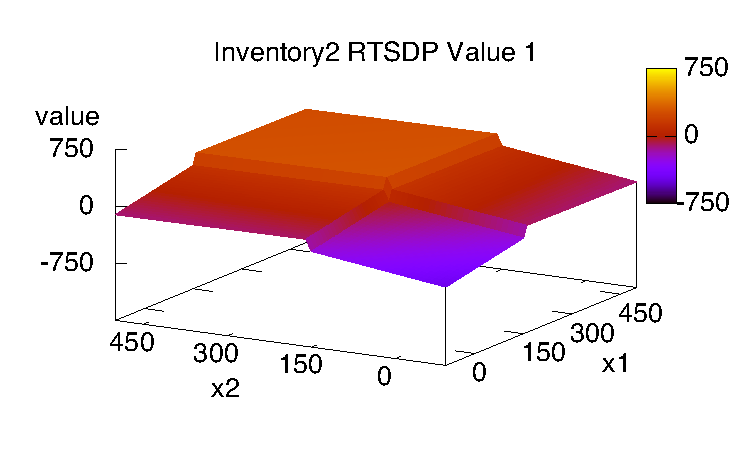
\includegraphics[width=0.26\linewidth, height=0.14\linewidth]{figures/\solutionExample/RTSDP-Value1.pdf}
\label{invent2rtdp_plot1}}
\subfloat[RTSDP - $DD^1$ - 7 Nodes]{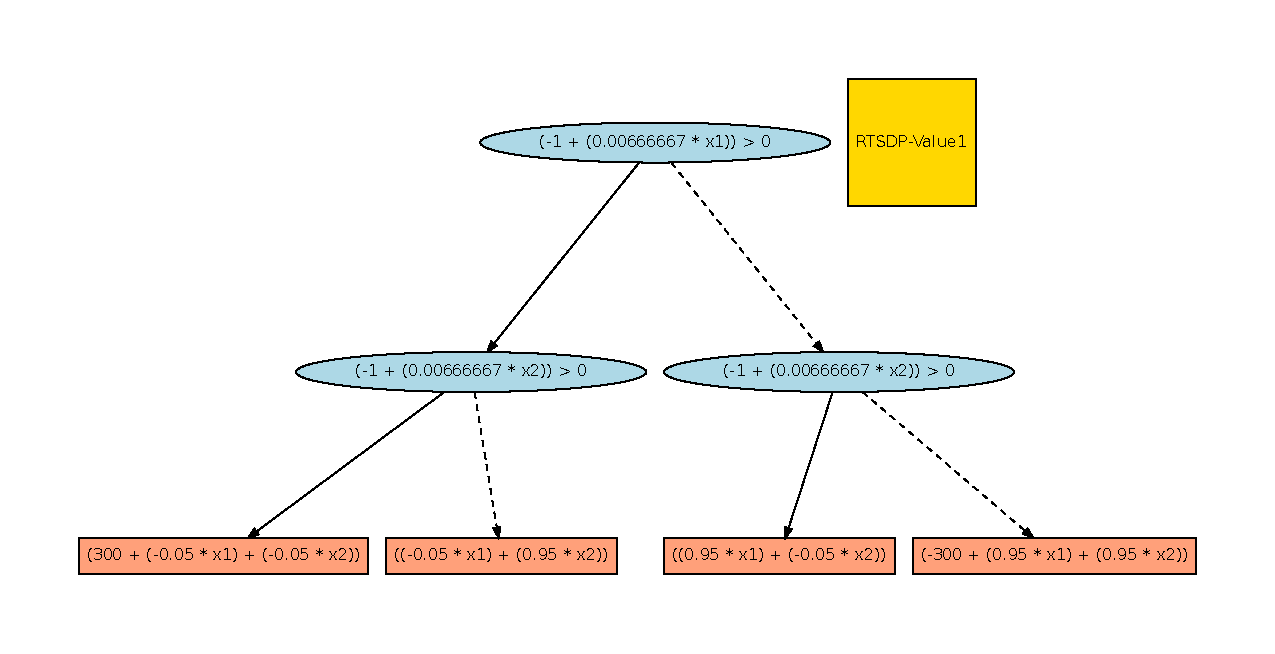
\includegraphics[width=0.22\linewidth, height=0.14\linewidth]{figures/\solutionExample/RTSDP-DD1.pdf}
\label{invent2rtdp_dd1}} 
\hspace{0.1cm}
\subfloat[SDP - $V^1$]{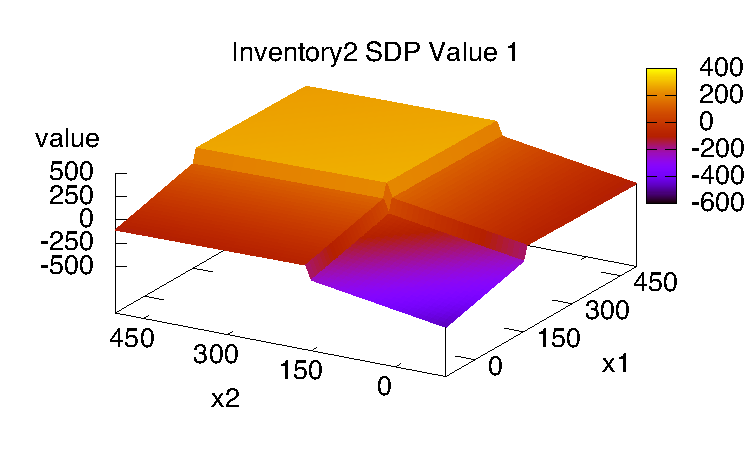
\includegraphics[width=0.26\linewidth, height=0.14\linewidth]{figures/\solutionExample/SDP-Value1.pdf}
\label{invent2sdp_plot1}}
\subfloat[SDP - $DD^1$ - 7 Nodes]{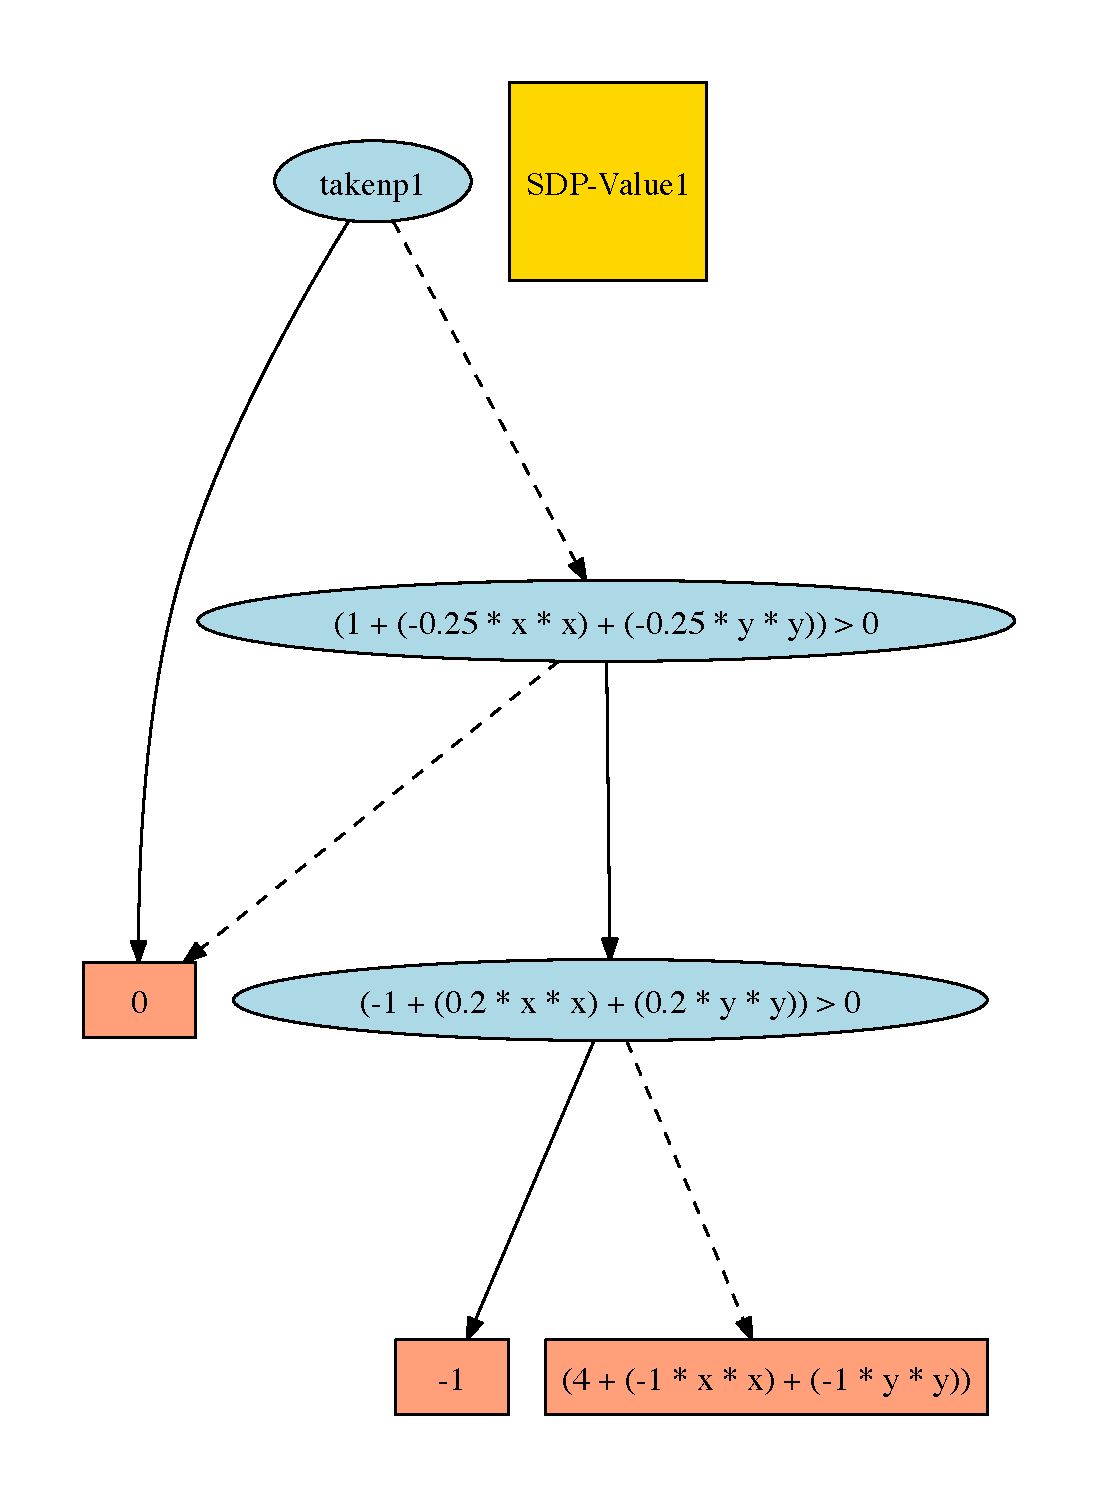
\includegraphics[width=0.22\linewidth, height=0.14\linewidth]{figures/\solutionExample/SDP-DD1.pdf}
\label{invent2sdp_dd1}} 

\subfloat[RTSDP - $V^2$]{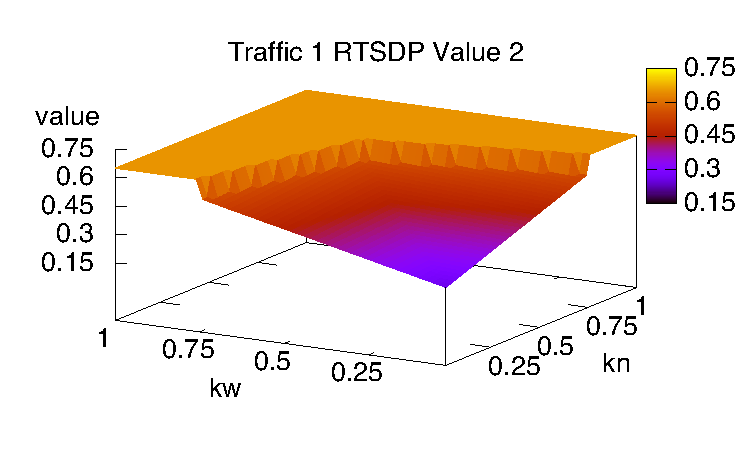
\includegraphics[width=0.26\linewidth, height=0.14\linewidth]{figures/\solutionExample/RTSDP-Value2.pdf}
\label{invent2rtdp_plot2}}
\subfloat[RTSDP - $DD^2$ - 22 Nodes]{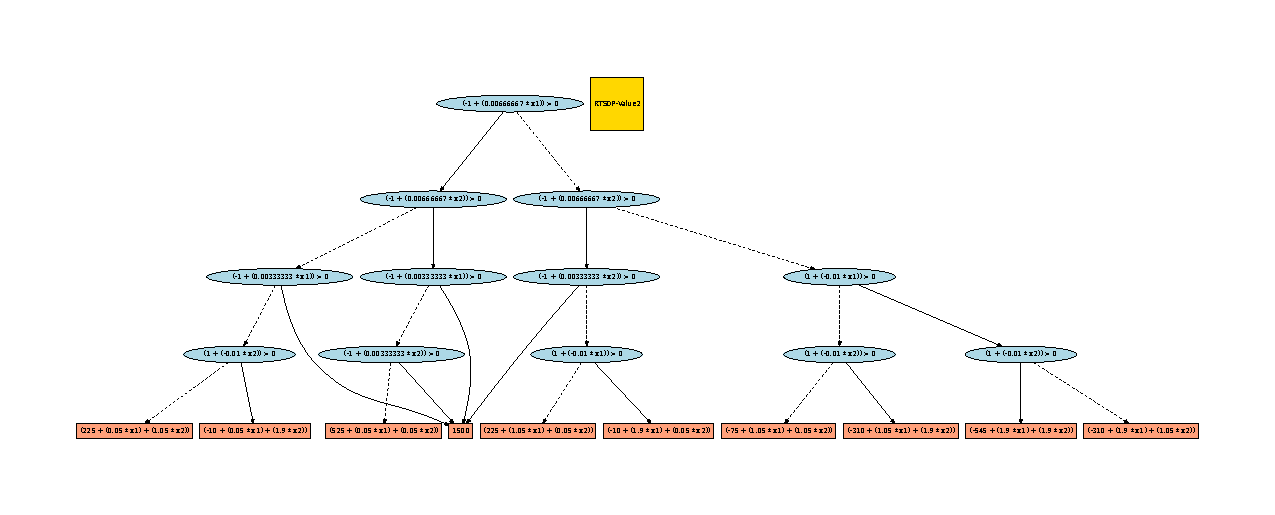
\includegraphics[width=0.22\linewidth, height=0.14\linewidth]{figures/\solutionExample/RTSDP-DD2.pdf}
\label{invent2rtdp_dd2}} 
\hspace{0.1cm}
\subfloat[SDP - $V^2$]{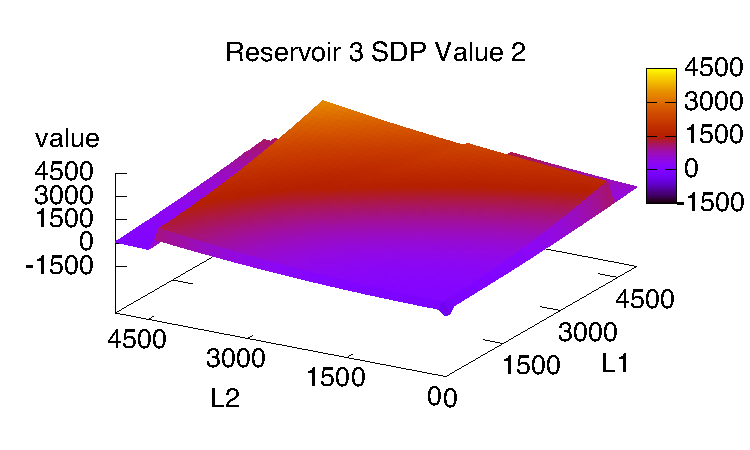
\includegraphics[width=0.26\linewidth, height=0.14\linewidth]{figures/\solutionExample/SDP-Value2.pdf}
\label{invent2sdp_plot2}}
\subfloat[SDP - $DD^2$ - 50 Nodes]{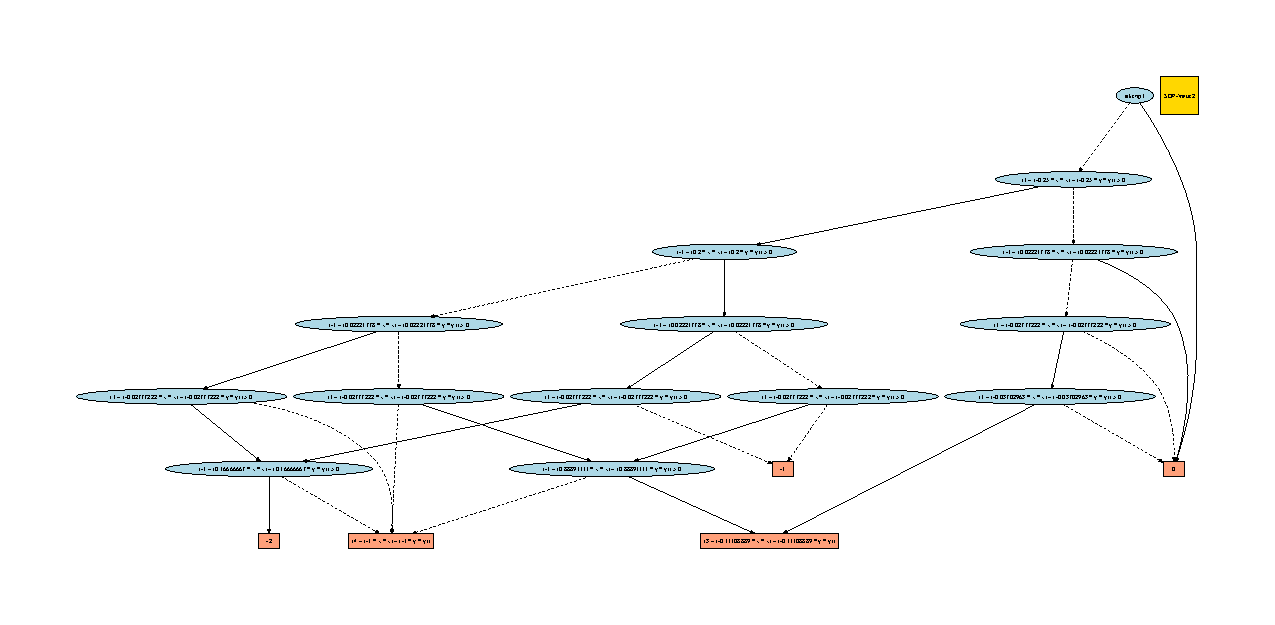
\includegraphics[width=0.22\linewidth, height=0.14\linewidth]{figures/\solutionExample/SDP-DD2.pdf}
\label{invent2sdp_dd2}} 

\subfloat[RTSDP - $V^3$]{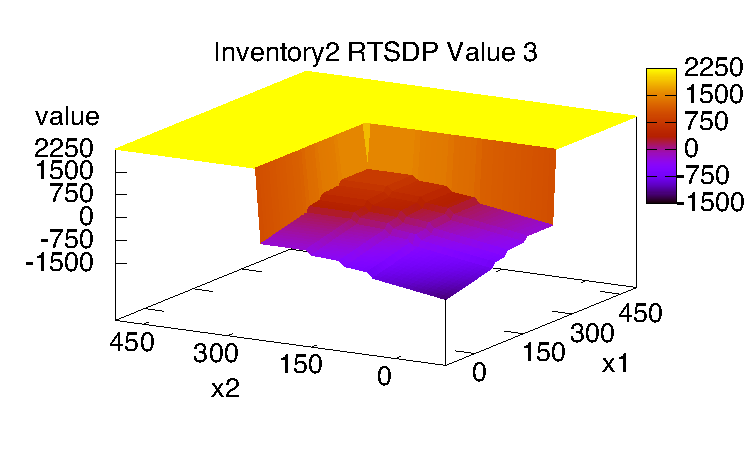
\includegraphics[width=0.26\linewidth, height=0.14\linewidth]{figures/\solutionExample/RTSDP-Value3.pdf}
\label{invent2rtdp_plot3}}
\subfloat[RTSDP - $DD^3$ - 39 Nodes]{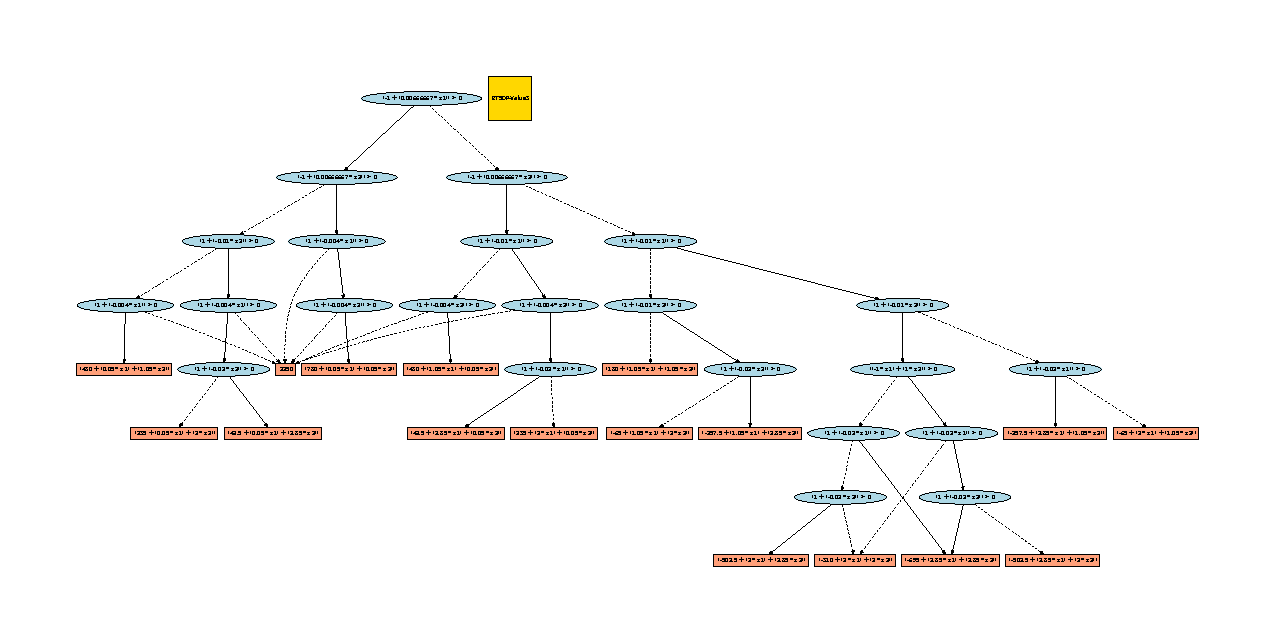
\includegraphics[width=0.22\linewidth, height=0.14\linewidth]{figures/\solutionExample/RTSDP-DD3.pdf}
\label{invent2rtdp_dd3}} 
\hspace{0.1cm}
\subfloat[SDP - $V^3$]{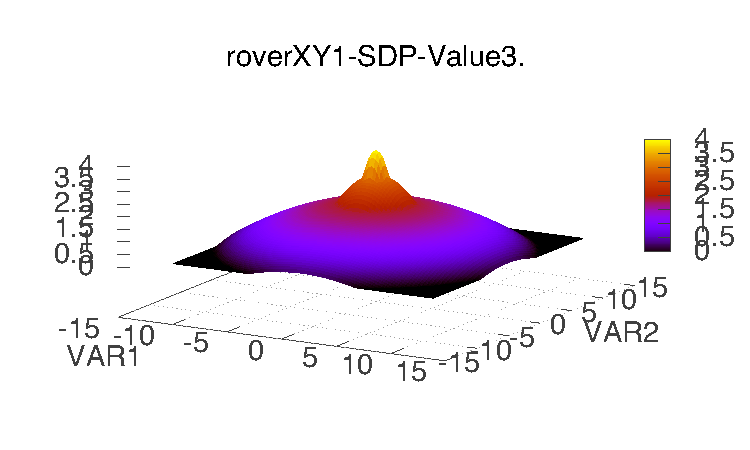
\includegraphics[width=0.26\linewidth, height=0.14\linewidth]{figures/\solutionExample/SDP-Value3.pdf}
\label{invent2sdp_plot3}}
\subfloat[SDP - $DD^3$ - 142 Nodes]{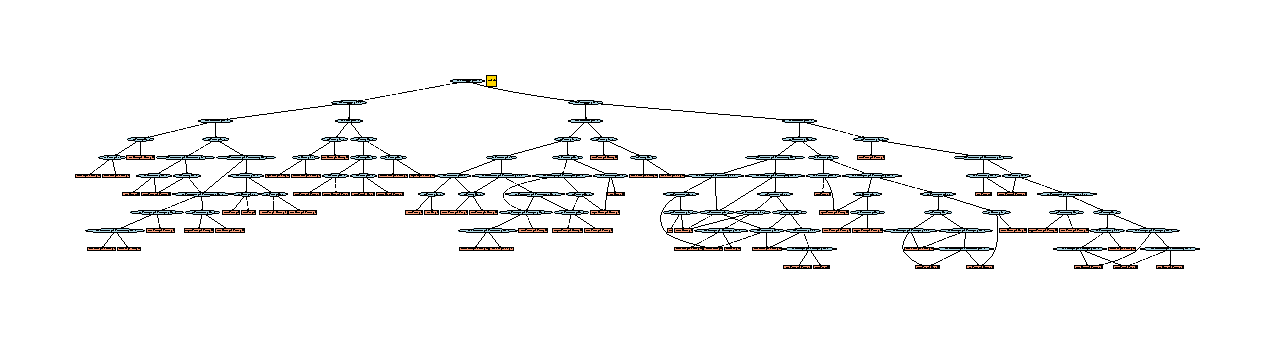
\includegraphics[width=0.22\linewidth, height=0.14\linewidth]{figures/\solutionExample/SDP-DD3.pdf}
\label{invent2sdp_dd3}} 

\subfloat[RTSDP - $V^4$]{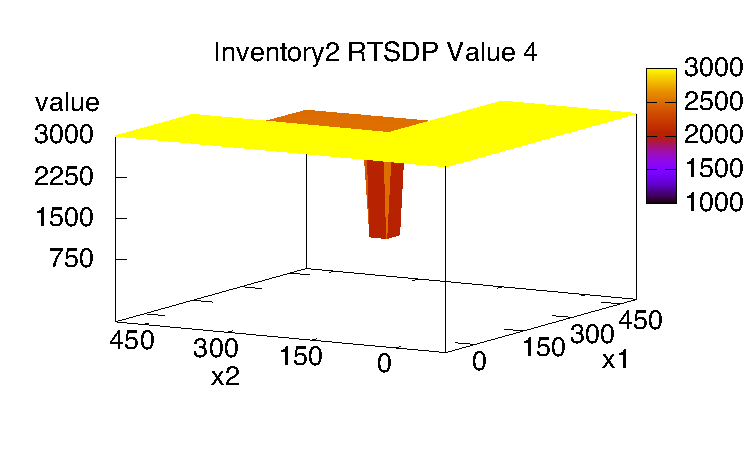
\includegraphics[width=0.26\linewidth, height=0.14\linewidth]{figures/\solutionExample/RTSDP-Value4.pdf}
\label{invent2rtdp_plot4}}
\subfloat[RTSDP - $DD^4$ - 12 Nodes]{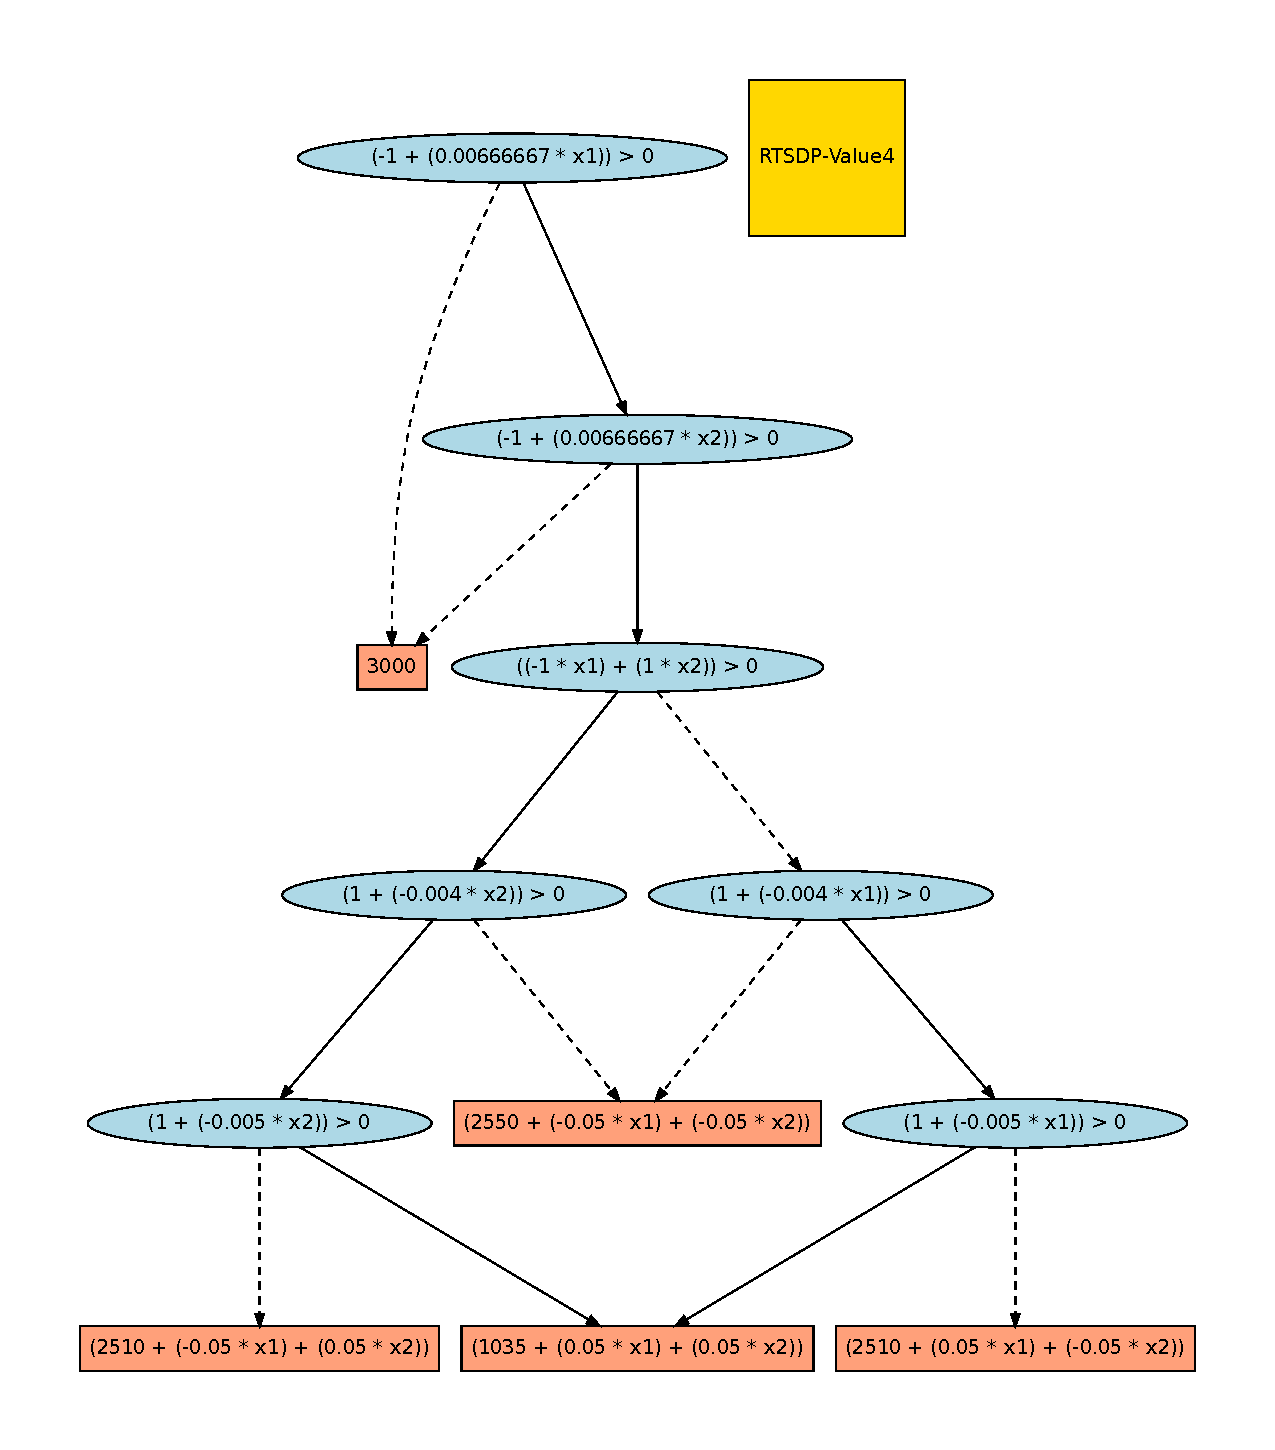
\includegraphics[width=0.22\linewidth, height=0.14\linewidth]{figures/\solutionExample/RTSDP-DD4.pdf}
\label{invent2rtdp_dd4}} 
\hspace{0.1cm}
\subfloat[SDP - $V^4$]{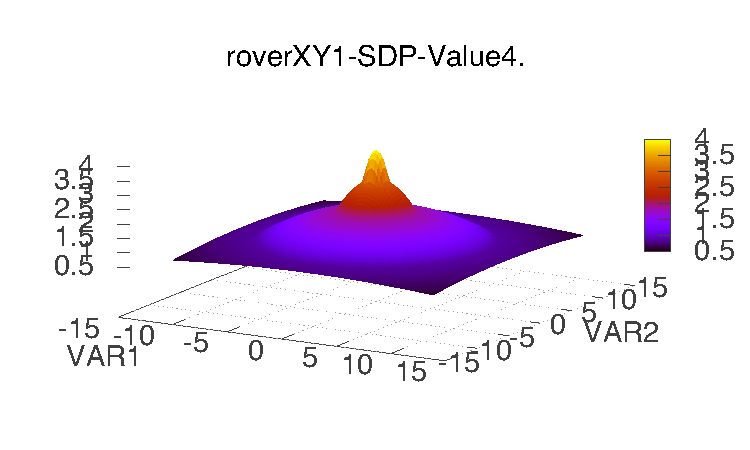
\includegraphics[width=0.26\linewidth, height=0.14\linewidth]{figures/\solutionExample/SDP-Value4.pdf}
\label{invent2sdp_plot4}}
\subfloat[SDP - $DD^4$ - 272 Nodes]{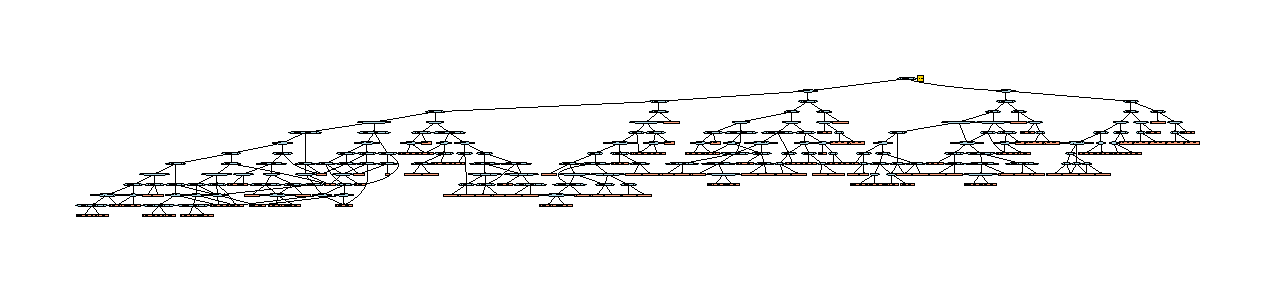
\includegraphics[width=0.22\linewidth, height=0.14\linewidth]{figures/\solutionExample/SDP-DD4.pdf}

\label{invent2sdp_dd4}} 
\caption{Value functions generated by RTSDP and SDP on \Invent, with $H=4$.}
\label{fig:solution}
\end{figure*}

Figure~\ref{fig:solution} shows the value functions for different stages-to-go generated by RTSDP \emph{(left)} and SDP \emph{(right)} when solving \Invent2, an instance with 2 continuous state variables and 2 continuous action parameters. The value functions are shown as 3D plots (value on the z axis as a function of continuous state variables on the x and y axes) with their corresponding XADDs. Note that the initial state is $(200,200)$ and that for this state the value found by RTSDP is the same as SDP. One observation is that the z-axis scale changes on every plot because both the reward and the upper bound heuristic increases with stages to-go.
Since RTSDP runs all trials from the initial state, the value function for $H$ stages-to-go, $V_H$ {\it (bottom)} is always updated on the same region: \emph{the one containing the initial state}.
The updates insert new decisions to the XADD, splitting the region containing $s_0$ into smaller regions, only the small region that still contains the initial state will keep being updated~(See Figure~\ref{invent2rtdp_plot4}).

An interesting observation is how the solution (XADD) size %(number of XADD nodes) 
changes for the different stages-to-go value functions. For SDP~(Figures \ref{invent2sdp_dd1}, \ref{invent2sdp_dd2}, \ref{invent2sdp_dd3} and \ref{invent2sdp_dd4}), the number of regions increases quickly with the number of actions-to-go (from top to bottom).
However, RTSDP~(Figures \ref{invent2rtdp_dd1}, \ref{invent2rtdp_dd2}, \ref{invent2rtdp_dd3} and \ref{invent2rtdp_dd4}) shows a different pattern: with few stages-to-go, the number of regions increases slowly with horizon, but for the target horizon (\ref{invent2rtdp_dd4}), the solution size is very small. This is explained because the number of reachable regions from the initial state in a few steps is small and therefore the number of terminal nodes and overall XADD size is not very large for greater stage-to-go, for instance, when the number of stages-to-go is the complete horizon the only reachable state (in 0 steps) is the initial state.
Note that this important difference in solution size is also reflected in the 3D plots, regions that are no longer relevant in a certain horizon stop being updated and remain with their upper bound heuristic value (e.g. the plateau with value 2250 at $V^3$).

\begin{table}[!ht]
\centering
%\small
\scriptsize
\begin{tabular}{c|cc|cc}
	\toprule
	Instance~(\#Cont.Vars)	 & \multicolumn{2}{c|}{SDP} & \multicolumn{2}{c}{RTSDP}  \\  \cmidrule{2-5}
	 & Time (s) & Nodes & Time (s) & Nodes \\ \midrule
	Inventory~1 (2)  & 0.97 & 43 & 1.03 & 37\\%4.6 & 123 & 77.3 & 230\\
	Inventory~2 (4) & 2.07 & 229 & 1.01 & 51\\
	Inventory~3 (6) & 202.5 & 2340 & 21.4 & 152\\ \bottomrule \toprule
%	Reservoir1  & 0.17 & 318 & 0.19 & 138\\
%	Reservoir2  & 0.227 & 440 & 0.26 & 184\\
%	Reservoir3  & 0.53 & 3476 & 0.47 & 657\\ \midrule %\footnote{Did Not Finish}
	Reservoir~1 (1) & \multicolumn{2}{c|}{Did not finish} & 1.6 & 1905\\
	Reservoir~2 (2) & \multicolumn{2}{c|}{Did not finish} & 11.7 & 7068\\
	Reservoir~3 (3) & \multicolumn{2}{c|}{Did not finish} & 160.3 & 182000\\ \bottomrule \toprule
%	Traffic1  & 0.05 & 28 & 0.06 & 28\\
%	Traffic2  & 0.075 & 63 & 0.078 & 48\\ \midrule \bottomrule \toprule
	Traffic~1 (4) & 204 & 533000 & 0.53 & 101\\
	Traffic~2 (5) & \multicolumn{2}{c|}{Did not finish} & 1.07 & 313\\ \bottomrule
\end{tabular}
\caption{\small Time and space comparison of SDP and RTSDP in various instances of the 3 domains.}
\label{tab:all}
\end{table}

Table \ref{tab:all} presents performance results of RTSDP and SDP in various instances of all domains. Note that the performance gap between SDP and RTSDP grows impressively with the number of continuous variables, because restricting the solution to relevant states becomes necessary. SDP is unable to solve most nonlinear problems since it cannot prune nonlinear regions, while RTSDP restricts expansions to visited states and has a much more compact value function.

\section{Conclusion}
We propose a new solution, the $RTSDP$ algorithm, for a general class of Hybrid MDP problems including linear dynamics with parametrized actions, as in \Invent, or nonlinear dynamics, as in \Traffic.
RTSDP uses the initial state information efficiently to (1) visit only a small fraction of the state space and (2) avoid representing infeasible nonlinear regions. In this way, it overcomes the two major drawbacks of SDP and greatly surpasses its performance into a more scalable solution for linear and nonlinear problems that greatly expand the set of domains where SDP could be used.
RTSDP can be further improved with better heuristics that may greatly reduce the  number of relevant regions in its solution. 
Such heuristics might be obtained using bounded approximate HMDP solvers \cite{vianna13}.

\section*{Acknowledgment}
This work has been supported by the Brazilian agency FAPESP (under 
 grant 2011/16962-0). NICTA is funded by the
 Australian Government as represented by
the Department of Broadband, Communications and the Digital
Economy and the Australian Research Council through the ICT
Centre of Excellence program.

\bibliography{mybib}
\bibliographystyle{aaai}
\end{document}